\section{Requirements Analysis}
Medical Problem, Theoretic background etc.

\subsection{Research}
The research effort is split into three logical parts:
\begin{itemize}
  \item Diabetes
  \item Food
  \item Insulin
\end{itemize}
Details to the specific part of interest are explained in the following section.

\subsubsection{Diabetes}

\subsubsection{Food}
There are two major "indexes" which try to relate the type of food to the foods effect on the blood sugar level (glucose level).
The first such index is the so called "Glycemic Index" (GI) the second one the "Glycemic Load" (GL).
The GL tries to take some criteria according to the GI in account which have been widely critizized.
Still the GL and especially GI are both still being controversially discussed by experts.
Most of this discussion as it appears is mainly because people tend to use
diets based on these indexes in order to try to effect blood sugar level
without medicine. For a rating in a simplified simulation these indexes should
work out well, though the GL may be the one to prefer as it addresses some
weaknesses of the GI \cite{norden:glycemicindex}.

The time needed for food to affect the blood sugar can roughly be splitted up
into three groups of food which affect blood sugar level fast, moderate or
slowly \cite{mit:glycemicindex}.

\paragraph{Simulation}
In order to simulate the glucose level increase, after food has been eaten, programatically, mathematical models have to be made in order to calculate this process.
Here it is focused on the three main types of different foods with respect to speed of their absorbtion (i.e. how fast the gluscose level rises after a meal).
These three main types split up in

\begin{itemize}
  \item high glycemic (fast),
  \item moderate glycemic (intermediate) and
  \item low glycemic (slow) foods.
\end{itemize}

Unfortunately there are no mathematical models available for simulating this.
So in order to make a somewhat sane simulation there is the suggestion to use different formulas in order to simulate the different behavior of this foods.
The type of formula choosen should represent the behavior of glucose level absorbtion / increase in an approximate way.
The ammount of the glucose increase and roughly the timespan it occours in can be influenced by variables in these formulas.
Fortunately at least rough estimates can be made according to the absorbtion of
glucose in the blood as there exists a table which associates different foods
with theire behavior according to CI, CL etc. \cite{glycemicindex:table}.

\paragraph{Formulas}
So far two formulas have been evaluated.
Formula a (see figure \vref{fig:food_function_a}) has no skew and therefore is
symmetric. \begin{figure}[htb]
\centering
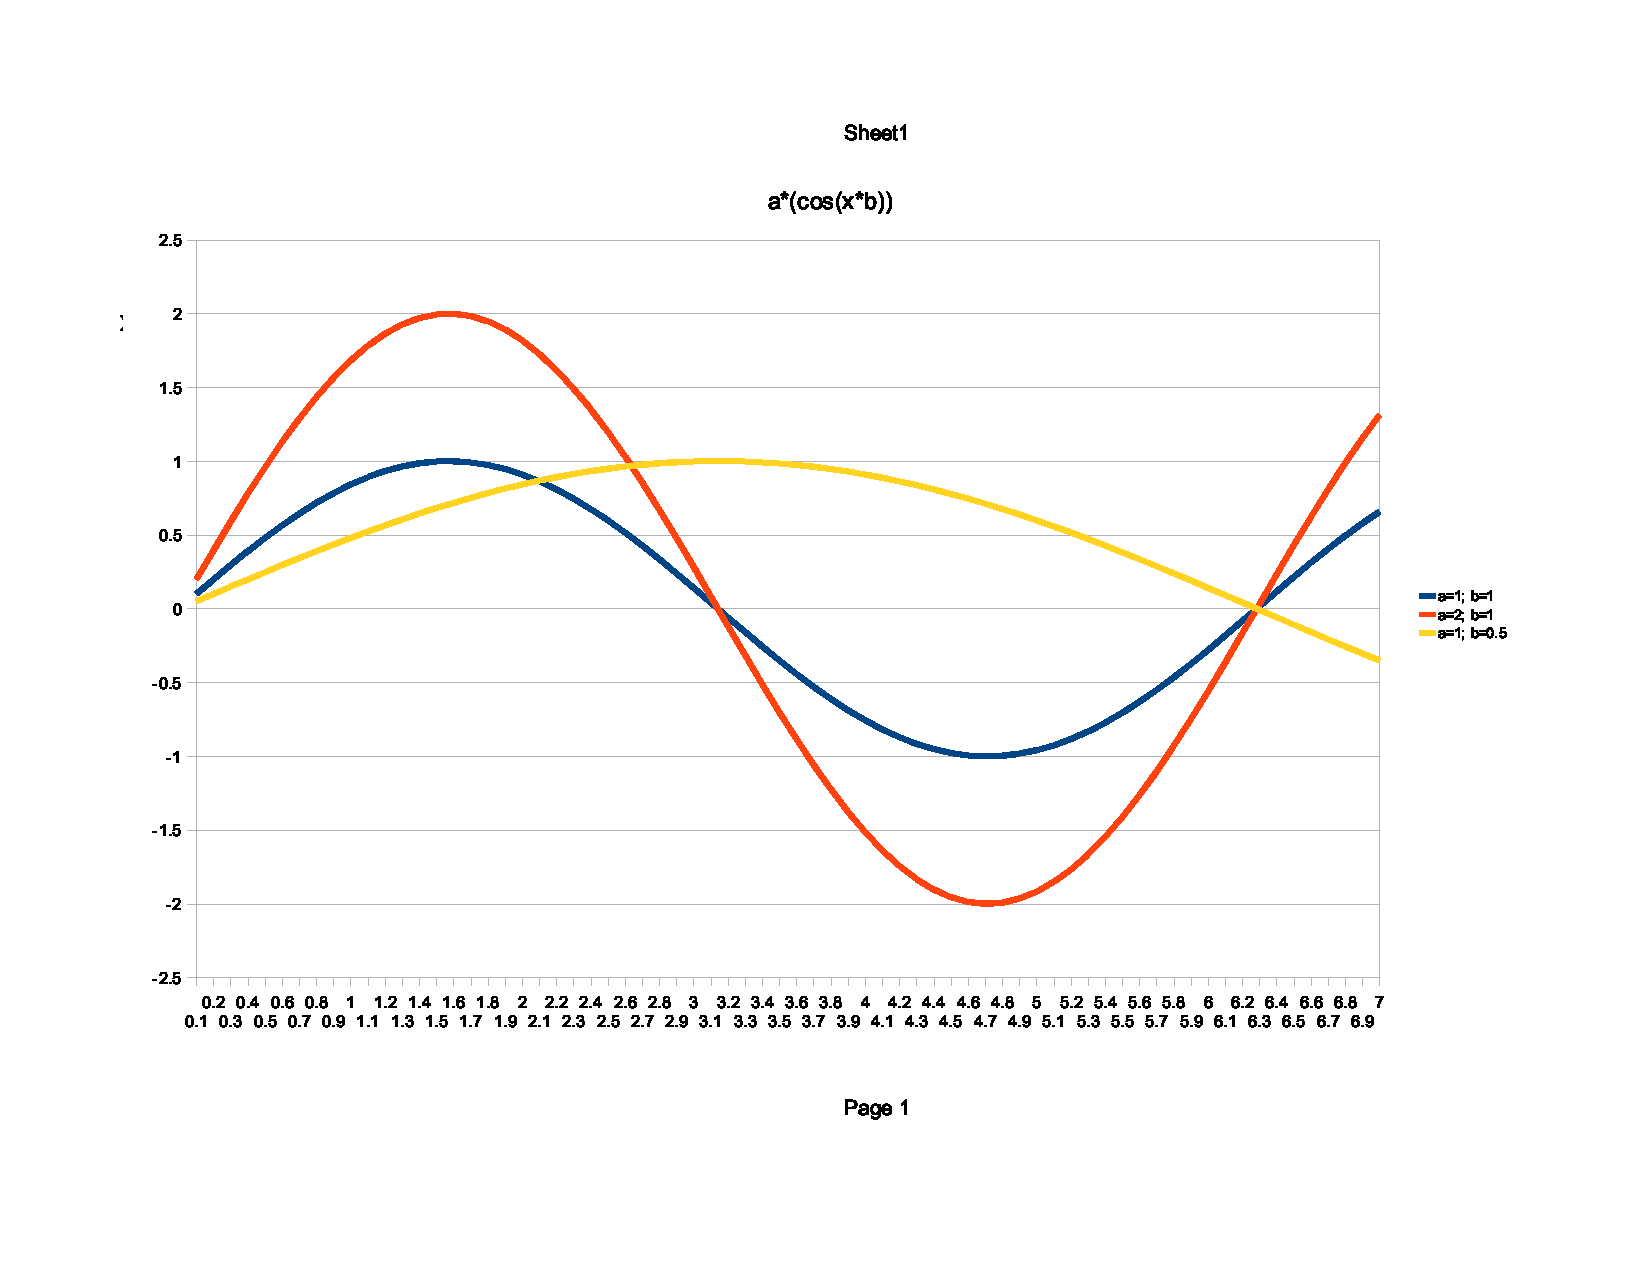
\includegraphics[width=\textwidth]{images/food_function_a}
\caption{Food Function A}
\label{fig:food_function_a}
\end{figure}
Formula b (see figure \vref{fig:food_function_b}) has a skew to the right. I.e.
it increases "slowly" two some point from which on it falls very abruptly. 
\begin{figure}[htb]
\centering
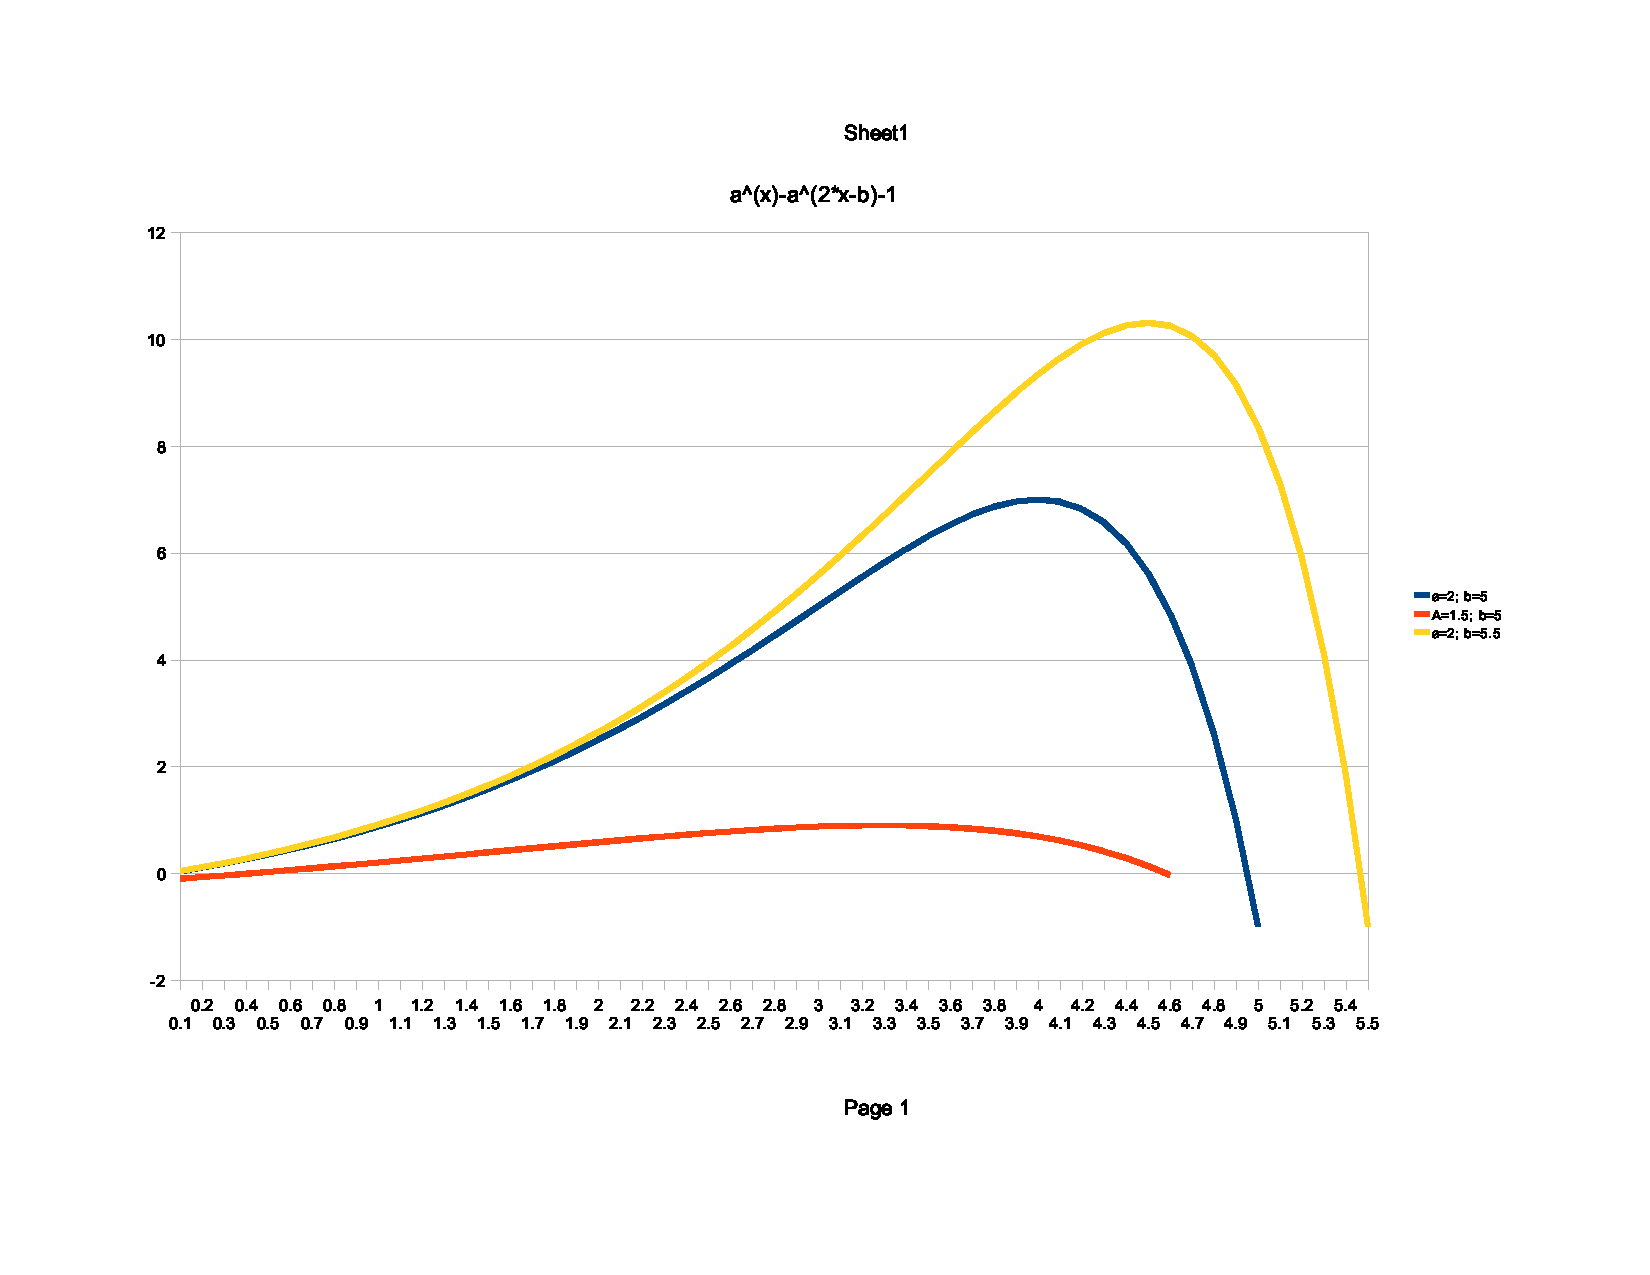
\includegraphics[width=\textwidth]{images/food_function_b}
\caption{Food Function B}
\label{fig:food_function_b}
\end{figure}
These formulas are attached with some sample data as Openoffice spread sheets under attachments.

\paragraph{Implementation}
In order to make it more flexible to choose different algorithms / formulas for
calculating the glucose values the Strategy pattern might be choosen. One
critical question with respect to the implementation is the choice of the used
data types for floatingpoint data as these data types are not guaranteed to be precise.

\subsubsection{Insulin}

\subsection{Requirements and Project Estimation}
The estimation of the project was done using COCOMO 2.
Therefore the metric used here is Lines Of Code (LOC).

First project estimation:
\begin{itemize}
  \item Behavior Simulation
  	\begin{itemize}
        \item eat (Guess: 450 LOC)
        \item insulin (Guess: 400 LOC)
        \item diabetes (Guess: 400 LOC)
    \end{itemize}
  \item Simulating Insulin Pump
  	\begin{itemize}
        \item actor (Insulin injection) (Guess: 600 LOC)
        \item sensor (Glucose Level Monitor) (Guess: 150 LOC)
        \item User Interface (Alarm/Input) (Guess: 500)
    \end{itemize}
\end{itemize} 
Guessed Estimation based on Experts Cocomo 2:
Effort 13.4 Person-months
Schedule 8.5 Months
\url{http://sunset.usc.edu/cgi-bin/expert_cocomo2000}